\documentclass[12pt]{article}
\usepackage{amsmath}
\usepackage{geometry}
\usepackage{graphicx}
\usepackage{hyperref}
\usepackage[latin1]{inputenc}
\usepackage{listings}
\renewcommand{\labelitemi}{$\textendash$}
\geometry{
    a4paper,
    total={170mm,257mm},
    left=15mm,
    right=15mm,
    top=5mm,
    bottom=15mm
}

\title{CS4061: Week 6 Assignment}
\author{Conor McCauley - 17323203}
\date{November 17, 2020}

\begin{document}

\maketitle

\noindent \textbf{Dataset Identifier:} \texttt{\# id:7-28-21}

\section*{Question (i)}

\noindent (a) In order to use different \textit{Gaussian} kernels when training our models we can use the following code to generate kernel lambda functions for particular values of $\gamma$ (this saves us the trouble of manually writing separate functions for each different value):

\begin{center}
    \lstset{basicstyle=\footnotesize}
    \begin{lstlisting}[language=Python]
    def generate_gaussian_kernel_function(gamma):
        weights = lambda dists: np.exp(-gamma * (dists ** 2))
        return lambda dists: weights(dists) / np.sum(weights(dists))
    \end{lstlisting}
\end{center}

For each $\gamma$ we can train our model and make predictions for values in the range $(-3, 3)$ using the following code:

\begin{center}
    \lstset{basicstyle=\footnotesize}
    \begin{lstlisting}[language=Python]
    kernel = generate_gaussian_kernel_function(gamma)
    model = KNeighborsRegressor(n_neighbors=3, weights=kernel).fit(X_train, Y_train)
    X_test = np.linspace(-3, 3, num=100).reshape(-1, 1)
    Y_pred = model.predict(X_test)
    \end{lstlisting}
\end{center}

Plotting these predictions along with the dummy training data results in the following:

\begin{center}
    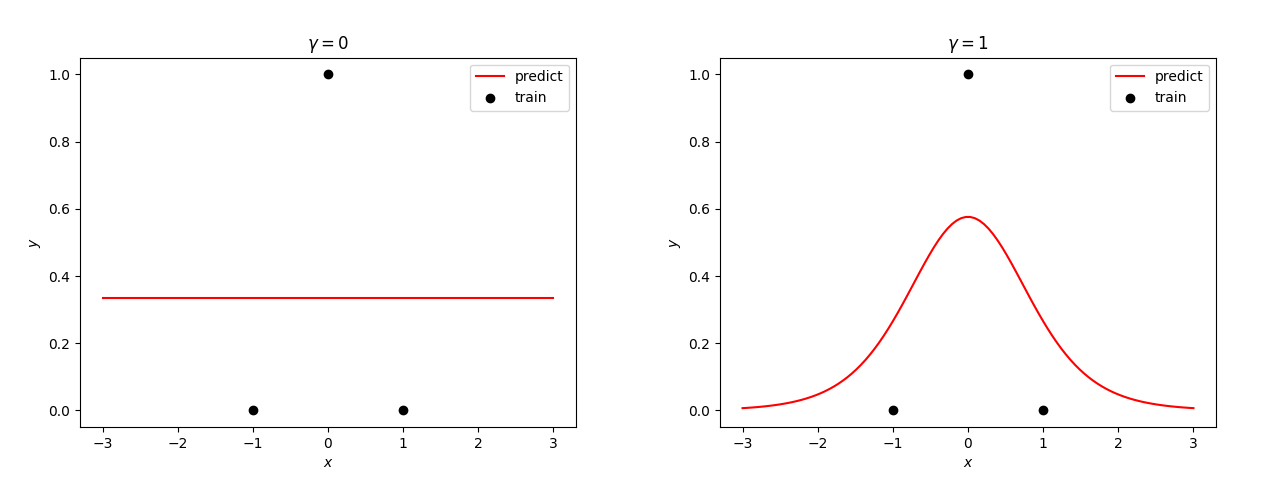
\includegraphics[scale=0.55]{fig_01a.png}
    
    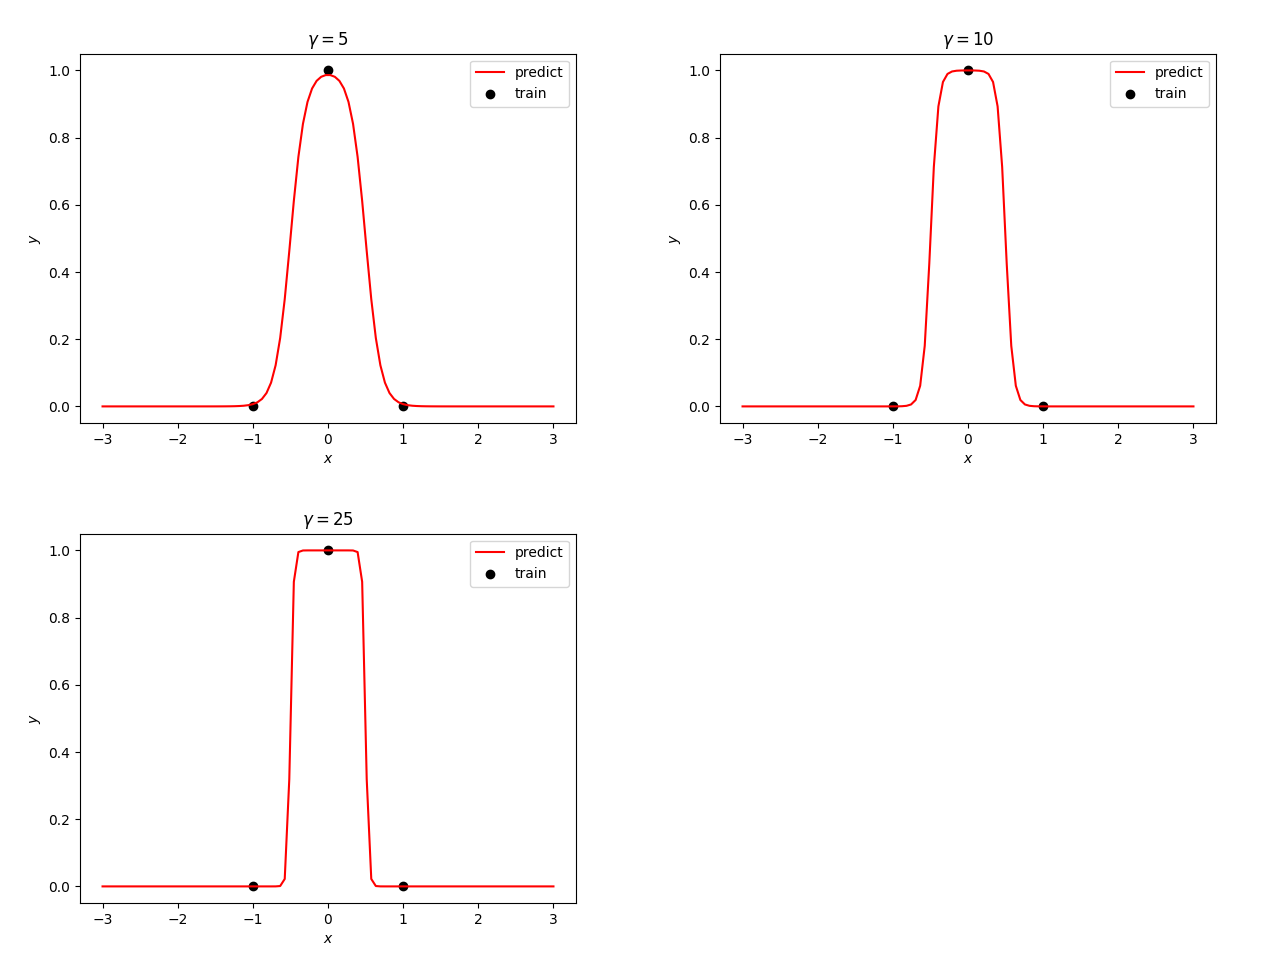
\includegraphics[scale=0.55]{fig_01b.png}
\end{center}

\noindent (b) A $k$NN linear regression model generates predictions for some new query point, $x$, by using the values of the $k$ training points that are closest (i.e., smallest Euclidean distance) to $x$ - the $k$ nearest neighbours. The predicted output value ultimately depends on how the distances to the $k$ nearest neighbours are weighted when calculating their mean. For example, if distances were weighted uniformly then all of the $k$ neighbours would have the same overall effect on the predicted output value. Alternatively, we can decrease the effect that points which are further away from $x$ would have using \textit{Gaussian} weighting. How much of an effect this distance will have on the weighted mean is determined by the $\gamma$ parameter.

Since we set $k = 3$ (the number of training points) all of our predictions will depend on the values of all of our training data. In our first plot $\gamma = 0$ meaning that no additional weight is given to nearer training points and, as such, all of our predictions are simply the mean output ($\frac{1+0+0}{3} = 0.33$). As we begin to increase the value of $\gamma$ we can see in the plots that the resulting predictions become smoother and begin to map to all of our training points.

However, when $\gamma$ is too large (e.g., $\gamma = 25$) the weighting given to the single closest training point becomes much larger than any other weighting which leads to the `curve' effectively snapping onto the nearest training point. This is why, for example, all predictions when $-0.5 < x < 0.5$ are exactly $1$ - only the second training point has any effect on the predicted value due to it being weighted much higher than the others.

\noindent (c) Using values of $C \in \{ 0.1, 1, 1000 \}$ and the same values of $\gamma$ from (a) we can use the following code to train each our models and make predictions for values in the range $(-3, 3)$:

\begin{center}
    \lstset{basicstyle=\footnotesize}
    \begin{lstlisting}[language=Python]
    model = KernelRidge(alpha=1/(2*C), kernel='rbf', gamma=gamma).fit(X_train, Y_train)
    X_test = np.linspace(-3, 3, num=100).reshape(-1, 1)
    Y_pred = model.predict(X_test)
    \end{lstlisting}
\end{center}

Plotting the resulting predictions along with the dummy training data produces the following:

\begin{center}
    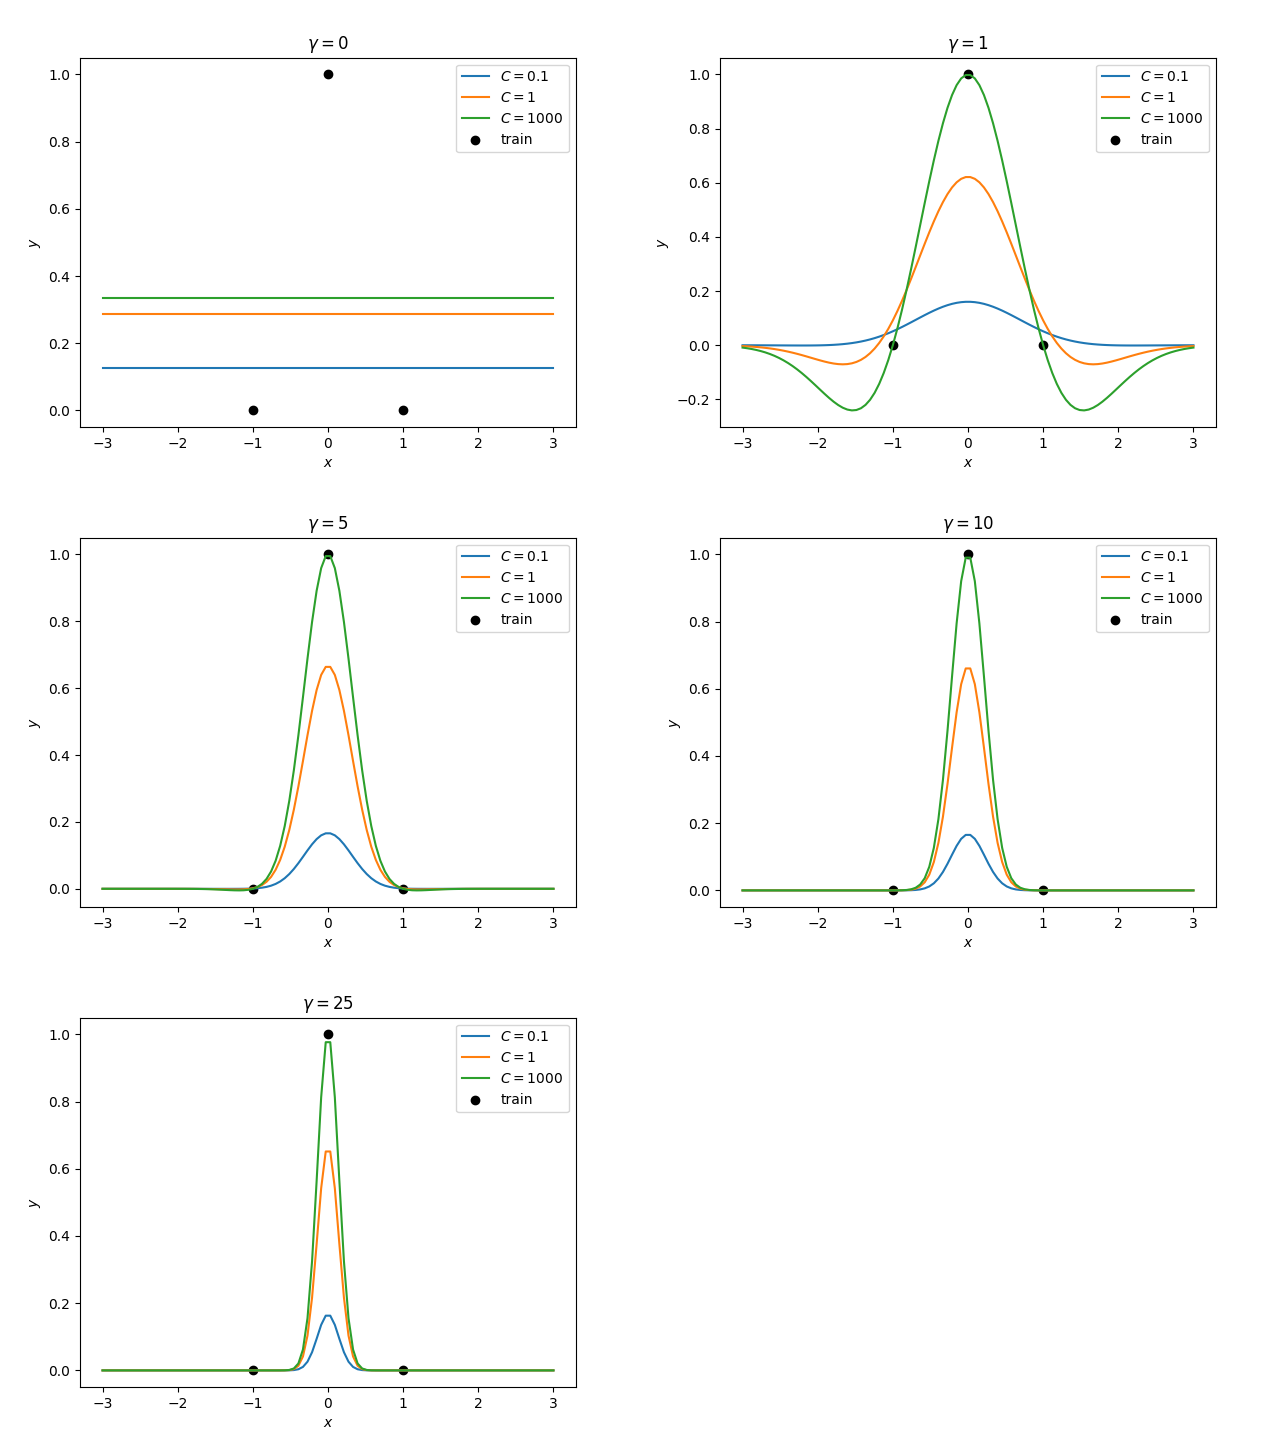
\includegraphics[scale=1.6]{fig_02.png}
\end{center}

The trained models reported the following dual coefficient parameters which we will discuss in (d):

\begin{center}
    \begin{tabular}{|c|c|c|c|}
        \hline
        $\gamma$ & $C = 0.1$ & $C = 1$ & $C = 1000$ \\
        \hline
        $0$ & $-0.025, 0.175, -0.025$ & $-0.571, 1.429, -0.571$ & $-666.6, 1333.4, -666.6$ \\
        $1$ & $-0.01, 0.168, -0.01$ & $-0.183, 0.757, -0.183$ & $-0.491, 1.361, -0.491$ \\
        $5$ & $0, 0.167, 0$ & $-0.003, 0.667, -0.003$ & $-0.007, 0.999, -0.007$ \\
        $10$ & $0, 0.167, 0$ & $0, 0.667, 0$ & $0, 0.999, 0$ \\
        $25$ & $0, 0.167, 0$ & $0, 0.667, 0$ & $0, 0.999, 0$ \\
        \hline
    \end{tabular}
\end{center}

\textbf{N.B.} while some of the values in the above table are zero this is solely due to my limiting each value to three decimal places - in actuality, while many of the values are very small, none of them are equal to zero.

\noindent (d) As is the case with a $k$NN model, a kernelised ridge regression (KRR) model uses the training points that are closest to a query point in order to make predictions. However, unlike a $k$NN model, the value of $k$ will always be equal to the number of training points. Our KRR model also uses a \textit{Gaussian} kernel with a $\gamma$ parameter to determine the weighting given to the different training points when making a prediction. The KRR will then train parameters $\theta$ on the kernel's data, like in standard linear regression, to generate a model that fits the training data - this model is trained using an $L_2$ regularisation penalty determined by the parameter $C$.

When $\gamma = 0$ the model is under-fitting and just predicting some form of overall mean value for each $C$. As we increase $\gamma$ we see that the model begins to fit the training data more effectively. However, even as we increase $\gamma$, it is clear that when $C = 0.1$ or $C = 1$ the model is under-fitting the training data leading to clearly incorrect predictions when $x = 0$. Out of the chosen values of $C$ it would seem that $C = 1000$ produces the best results. As was also the case with our $k$NN model, when $\gamma$ becomes too large our model also begins putting a bit too much weight on the training point closest to the query point.

If we look at the reported dual coefficient parameters we can see that as $C$ is increased the less important features get closer to zero while the most important feature increases in value. This important feature seems to correspond with the second training point. Furthermore, as $\gamma$ increases this effect becomes more pronounced due to the additional weight given to the closest training point.

The KRR model does not snap its predictions to the nearest training point to the same extent as the $k$NN model resulting in a smoother predictive curve in most cases. However, the accuracy of the predictions made by the KRR model depend quite heavily on the value of $C$.

\section*{Question (ii)}

\noindent (a) The code used in this question to train our $k$NN models is almost identical to the code used in (i) and, as such, I will not repeat any of the explanation/snippets I gave in (i).

Predictions will be made for values in the range $(-3, 3)$ and the following $\gamma$ values will be used: $\gamma \in \{0, 1, 5, 10, 25, 50, 100\}$.

\begin{center}
    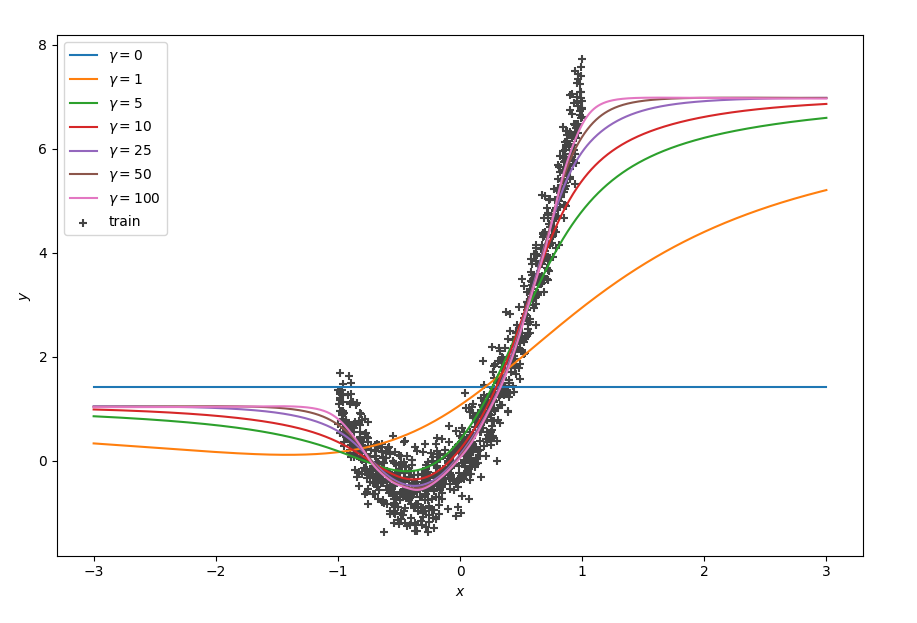
\includegraphics[scale=0.75]{fig_03.png}
\end{center}

As discussed in (i), when $\gamma = 0$ the distance between the query point and the neighbouring training points has no effect on the resulting prediction and, as such, the result is simply the mean value of the neighbouring points (which, in our case, is the mean of the entire dataset). As we increase $\gamma$ training points that are closer to our query points begin to have more and more of an effect on the overall prediction while training points that are further away play less of a role. For example, when $\gamma = 1$ points that are further away still have quite a bit of impact on predictions and the resulting curve looks nothing like our training data. However, for greater values of $\gamma$ the predictive curves get closer and closer to our training data.

At the lower and upper bounds of our training data it can be seen that the predictions diverge entirely from our training data and simply predict constant values (much like when $\gamma = 0$). This is due to the fact that there are no individual clusters of training points that are particularly close to these query points; the resulting predictions are essentially a rough mean of the training points at either extreme end of the training data (around 1 at the lower end and around 7 at the upper end). As $\gamma$ increases this effect becomes more pronounced due to training points further from the extremes having even less of an effect.

\noindent (b) Using code that is almost identical to the code in (i) we can train KRR models for the following $\gamma$ and $C$ values: $\gamma \in \{0, 1, 5, 10, 25, 50, 100\}, C \in \{0.1, 1, 10, 1000\}$. We can then make predictions for values in the range $(-3, 3)$ which result in the following plots:

\begin{center}
    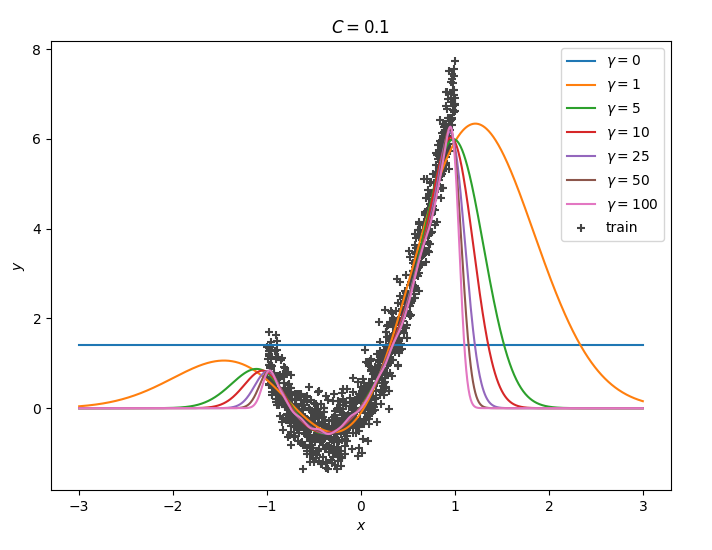
\includegraphics[scale=0.75]{fig_04.png}
    
    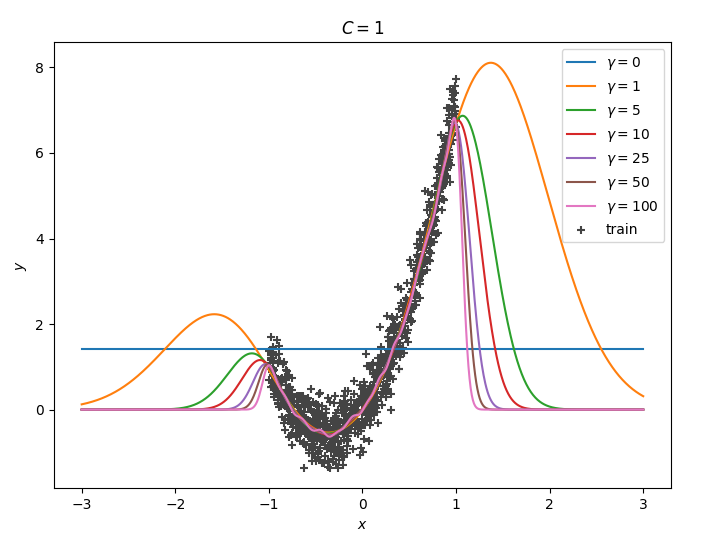
\includegraphics[scale=0.75]{fig_05.png}
    
    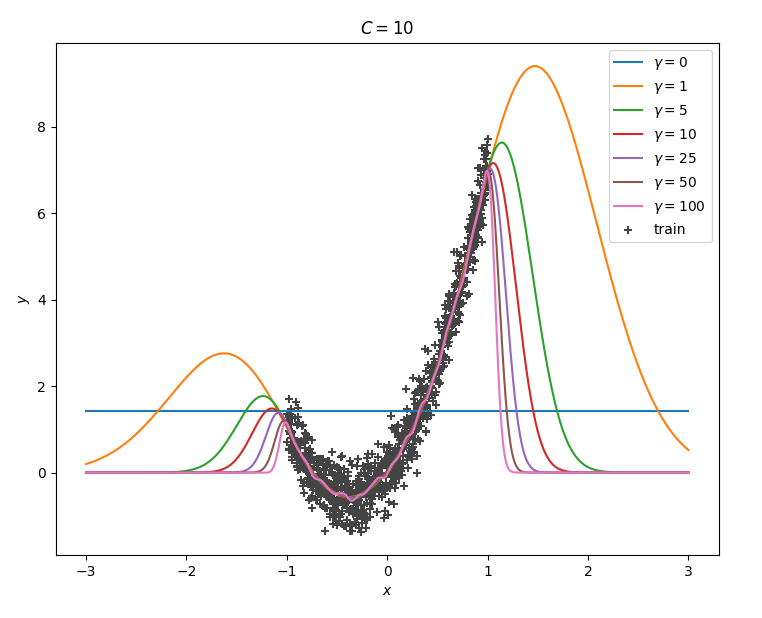
\includegraphics[scale=0.7]{fig_06.png}
    
    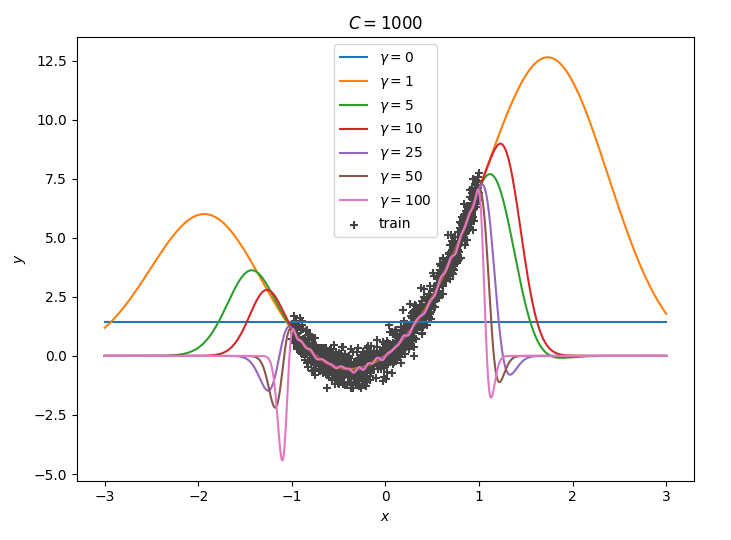
\includegraphics[scale=0.75]{fig_07.png}
\end{center}

As discussed in (i), when $\gamma = 0$ the model is under-fitting and predicting some mean value. Again, as previously discussed in (i), as $\gamma$ is increased the effect that closer training points have on the predictions becomes more pronounced and the curve resulting from the predictions becomes closer and closer to the one we would expect from the training data. However, when $\gamma$ becomes too large (i.e., $\gamma = 100$) it is clear that the model has begun to over-fit and is most likely factoring random noise into the predictions - this is evident given the minor fluctuations that occur in the otherwise smooth curve in the $(-1, 0.5)$ range.

\noindent (c) In order to choose an optimal $\gamma$ value for our $k$NN model we can use 5-fold cross-validation to plot the mean square error (MSE) and standard deviation (SD) for each $\gamma$. We will compare our models with a baseline that always predicts the mean value.

We can use a \texttt{DummyRegressor} to calculate the MSE for the baseline model like so:

\begin{center}
    \lstset{basicstyle=\footnotesize}
    \begin{lstlisting}[language=Python]
    dummy = DummyRegressor(strategy='mean').fit(X_train, Y_train)
    dummy_scores = cross_val_score(dummy, X_train, Y_train, cv=5
        scoring='neg_mean_squared_error')
    dummy_mean, dummy_std = dummy_scores.mean(), dummy_scores.std()
    \end{lstlisting}
\end{center}

In order to calculate the MSE and SD for our trained models we can use the following code (note how we must specify the number of neighbours in our model to be four-fifths the total size of our dataset):

\begin{center}
    \lstset{basicstyle=\footnotesize}
    \begin{lstlisting}[language=Python]
    gammas = [0, 1, 5, 10, 25, 50, 100]
    means, stds = [], []
    for gamma in gammas:
        kernel = generate_gaussian_kernel_function(gamma)
        model = KNeighborsRegressor(n_neighbors=int(len(X_train) * 0.8), weights=kernel)
            .fit(X_train, Y_train)
        scores = cross_val_score(model, X_train, Y_train, cv=5,
            scoring='neg_mean_squared_error')
        means.append(scores.mean())
        stds.append(scores.std())
    \end{lstlisting}
\end{center}

This produces the following plot:

\begin{center}
    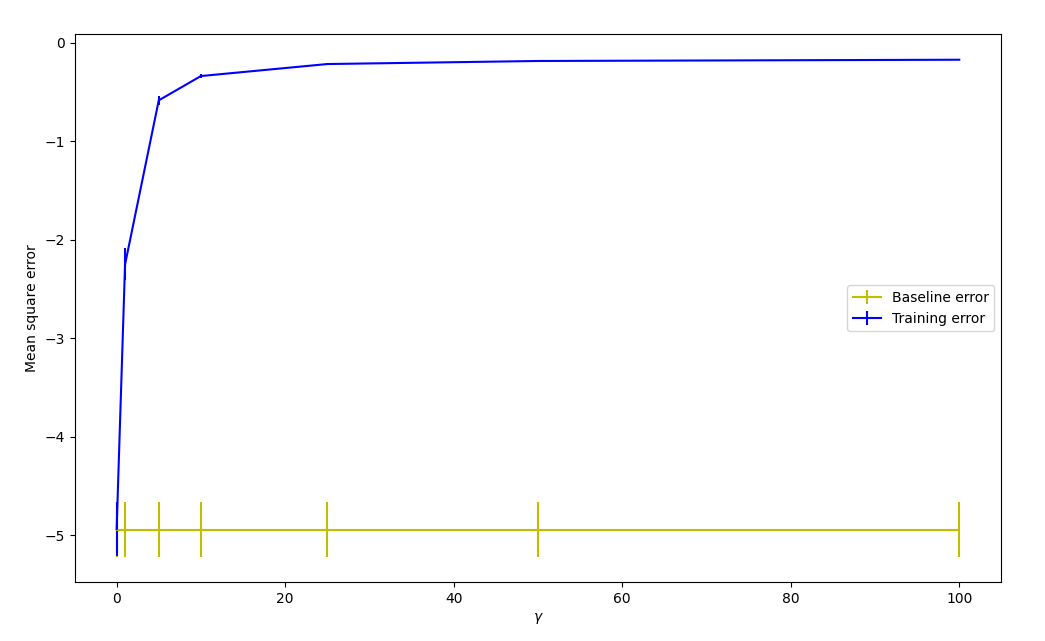
\includegraphics[scale=0.6]{fig_08.png}
\end{center}

As the above plot is a quite difficult to read I've also included the following much clearer plot which contains the results for the trained model when $\gamma \ge 5$:

\begin{center}
    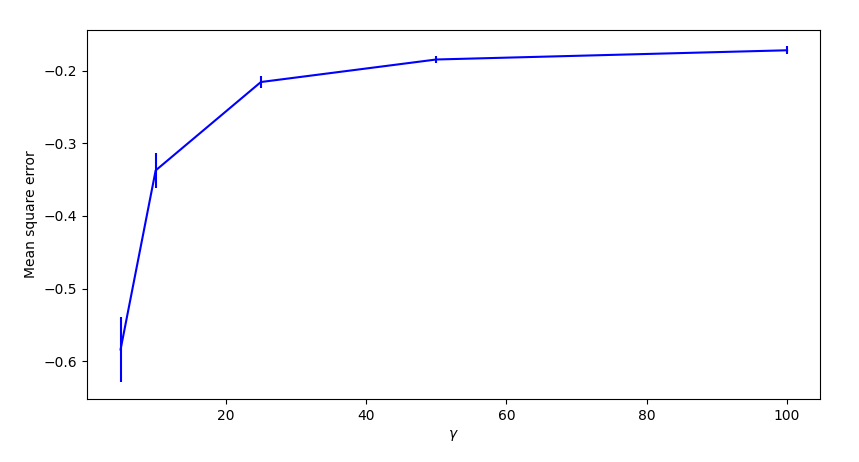
\includegraphics[scale=0.7]{fig_09.png}
\end{center}

Based on the first plot we can immediately dismiss both $\gamma = 0$ and $\gamma = 1$ as they both perform very poorly compared to larger $\gamma$ values. Looking at the second plot we can see that $\gamma = 5$ and $\gamma = 10$ both perform much worse than their larger counterparts - in both MSE and SD - so we can also dismiss them. The exact error values of the three remaining options are as follows:

\begin{center}
    \begin{tabular}{|c|c|c|}
        \hline
        $\gamma$ & MSE & SD \\
        \hline
        $25$ & $-0.215$ & $0.009$ \\
        $50$ & $-0.184$ & $0.004$ \\
        $100$ & $-0.172$ & $0.005$ \\
        \hline
    \end{tabular}
\end{center}

It is clear that both $\gamma = 50$ and $\gamma = 100$ perform slightly better than $\gamma = 25$ in both MSE and SD. $\gamma = 100$ has a slightly better MSE but an SD that is slightly larger. Nonetheless, looking at both the reported error values as well as the predictions plot from (a) it would seem that a value of $\gamma = 100$ would be the optimal choice here.

In order to choose optimal values for $\gamma$ and $\alpha$ for our KRR model we will again use 5-fold cross-validation to plot the mean square errors. We will also make use of the same baseline model for comparison. We can use the following code to calculate MSE and SD for each value of $\gamma$ and $C$:

\begin{center}
    \lstset{basicstyle=\footnotesize}
    \begin{lstlisting}[language=Python]
    C_range = [0.1, 1, 10, 1000]
    gammas = [0, 1, 5, 10, 25, 50, 100]
    for C in C_range:
        means, stds = [], []
        for gamma in gammas:
            model = KernelRidge(alpha=1/(2*C), kernel='rbf', gamma=gamma)
                .fit(X_train, Y_train)
            scores = cross_val_score(model, X_train, Y_train, cv=k,
                scoring='neg_mean_squared_error')
            means.append(scores.mean())
            stds.append(scores.std())
    \end{lstlisting}
\end{center}

As was the case with the $k$NN model the resulting plot is quite difficult to read:

\begin{center}
    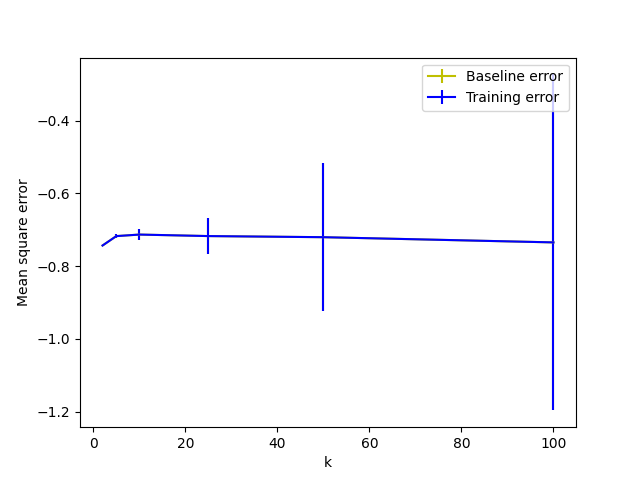
\includegraphics[scale=0.75]{fig_10.png}
\end{center}

The following plot, which does not include the baseline model and only contains results where $\gamma \ge 1$, is much clearer:

\begin{center}
    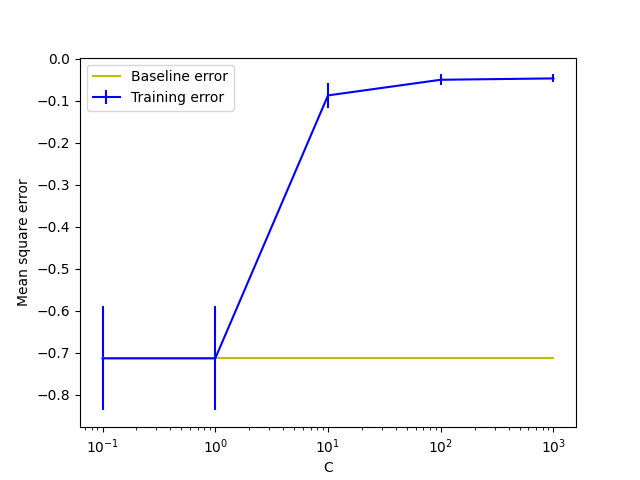
\includegraphics[scale=0.75]{fig_11.png}
\end{center}

Based on the first plot we can immediately dismiss $\gamma = 0$ for all $C$ values as it does not perform any better than our baseline model. From the second plot we can also dismiss $C = 0.1$ as it performs worse than all other values of $C$ irrespective of $\gamma$.

We can also ignore any values of $\gamma > 10$ as, not only do they almost always perform slightly worse than smaller values of $\gamma$ in both MSE and SD but we could see from the plots in (b) that they appeared to be over-fitting the dataset and allowing random noise to influence their predictions. The exact error values of the remaining $\gamma$ and $C$ values are as follows:

\begin{center}
    \begin{tabular}{|c|c|c|c|}
        \hline
        $C$ & $\gamma$ & MSE & SD \\
        \hline
        $1$ & $1$ & $-0.168$ & $0.006$ \\
        $1$ & $5$ & $-0.164$ & $0.008$ \\
        $1$ & $10$ & $-0.163$ & $0.008$ \\
        $10$ & $1$ & $-0.160$ & $0.010$ \\
        $10$ & $5$ & $-0.161$ & $0.011$ \\
        $10$ & $10$ & $-0.161$ & $0.011$ \\
        $1000$ & $1$ & $-0.160$ & $0.012$ \\
        $1000$ & $5$ & $-0.161$ & $0.012$ \\
        $1000$ & $10$ & $-0.163$ & $0.012$ \\
        \hline
    \end{tabular}
\end{center}

Given how similar all of these values are to one another it doesn't seem to be too important which parameters we choose. Nonetheless, it would seem that either $(C = 1, \gamma = 10)$ or $(C = 10, \gamma = 1)$ would be the best choices given their slightly better values in SD and MSE, respectively. Of the two options the latter might be the most optimal choice since it's got a slightly smaller MSE. Therefore, our optimal parameters are $\alpha = 1/2C = 0.05, \gamma = 1$.

The exact error values of our optimised models and our baseline model were as follows:

\begin{center}
    \begin{tabular}{|c|c|c|}
        \hline
        Model & MSE & SD \\
        \hline
        $k$NN & $-0.172$ & $0.005$ \\
        KRR & $-0.160$ & $0.010$ \\
        Baseline & $-4.941$ & $0.277$ \\
        \hline
    \end{tabular}
\end{center}

We can compare the predictions of our optimised $k$NN and KRR models (as well as our baseline model) for values in the extended range $(-3, 3)$ in the following plot:

\begin{center}
    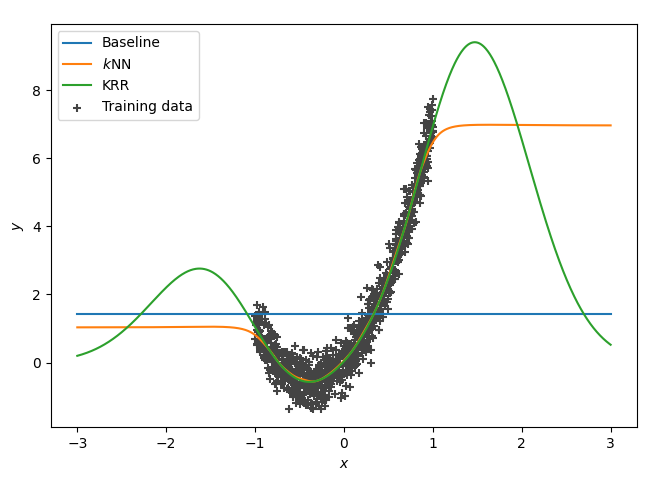
\includegraphics[scale=0.75]{fig_12.png}
\end{center}

For values in the general range $(-1, 1)$ both of the models appear to make very accurate predictions. However, as mentioned previously, the $k$NN model begins to predict constant values for values outside the range of the training data. The KRR model does not do this and appears to be predict values in what appears to be a more accurate manner. The KRR model also makes more accurate predictions for values in the dataset that are quite close to the extremes. Based on these observations, as well as its slightly better MSE, it seems that the KRR model is the better choice for this dataset. However, one caveat worth noting when choosing the KRR model is that for more extreme values in the extended range, i.e., $x < -2.5, x > 2$, the  predicted values begin to taper off and may in fact be less accurate than the constant predictions of the $k$NN model.

\section*{Appendix: Code}

\lstset{basicstyle=\footnotesize}
\begin{lstlisting}[language=Python]
from sklearn.dummy import DummyRegressor
from sklearn.kernel_ridge import KernelRidge
from sklearn.model_selection import cross_val_score
from sklearn.neighbors import KNeighborsRegressor
import matplotlib.pyplot as plt
import numpy as np
import pandas as pd

# generate a lambda kernel function for a given gamma value rather than 
#   manually writing seperate functions for each gamma value
def generate_gaussian_kernel_function(gamma):
    weights = lambda dists: np.exp(-gamma * (dists ** 2))
    return lambda dists: weights(dists) / np.sum(weights(dists))

# select specific feature from the data
def filter_data(data, index):
    return [d[index] for d in data]

def part_i_a(X_train, Y_train):
    gammas = [0, 1, 5, 10, 25]
    for gamma in gammas:
        # train model and make predictions
        kernel = generate_gaussian_kernel_function(gamma)
        model = KNeighborsRegressor(n_neighbors=3, weights=kernel).fit(X_train, Y_train)
        X_test = np.linspace(-3, 3, num=100).reshape(-1, 1)
        Y_pred = model.predict(X_test)
        # plot training data and predictions
        plt.scatter(X_train, Y_train, color='black')
        plt.plot(X_test, Y_pred, color='red')
        plt.xlabel('$x$')
        plt.ylabel('$y$')
        plt.legend(['predict', 'train'])
        plt.title(f'$\\gamma = {gamma}$')
        plt.show()

def part_i_c(X_train, Y_train):
    X_test = np.linspace(-3, 3, num=100).reshape(-1, 1)
    gammas = [0, 1, 5, 10, 25]
    C_range = [0.1, 1, 1000]
    for gamma in gammas:
        for C in C_range:
            # train model and make predictions
            model = KernelRidge(alpha=1/(2*C), kernel='rbf', gamma=gamma)
                .fit(X_train, Y_train)
            Y_pred = model.predict(X_test)
            plt.plot(X_test, Y_pred)
            print(
                'gamma = %d, C = %d, coefs = (%.5f, %.5f, %.5f)' %
                (gamma, C, model.dual_coef_[0][0], model.dual_coef_[1][0],
                    model.dual_coef_[2][0])
            )
        # configure and show plot
        plt.scatter(X_train, Y_train, color='black')
        plt.xlabel('$x$')
        plt.ylabel('$y$')
        plt.legend(['$C = 0.1$', '$C = 1$', '$C = 1000$', 'train'])
        plt.title(f'$\\gamma = {gamma}$')
        plt.show()
    return

def part_ii_a(X_train, Y_train):
    legend = []
    gammas = [0, 1, 5, 10, 25, 50, 100]
    for gamma in gammas:
        # train model and make predictions
        kernel = generate_gaussian_kernel_function(gamma)
        model = KNeighborsRegressor(n_neighbors=len(X_train), weights=kernel)
            .fit(X_train, Y_train)
        X_test = np.linspace(-3, 3, num=1000).reshape(-1, 1)
        Y_pred = model.predict(X_test)
        plt.plot(X_test, Y_pred)
        legend.append(f'$\\gamma = {gamma}$')
    # configure and show plot
    plt.scatter(X_train, Y_train, color='#444444', marker='+')
    legend.append('train')
    plt.xlabel('$x$')
    plt.ylabel('$y$')
    plt.legend(legend)
    plt.show()

def part_ii_b(X_train, Y_train):
    legend = []
    C_range = [0.1, 1, 10, 1000]
    gammas = [0, 1, 5, 10, 25, 50, 100]
    for C in C_range:
        for gamma in gammas:
            # train model and make predictions
            model = KernelRidge(alpha=1/(2*C), kernel='rbf', gamma=gamma)
                .fit(X_train, Y_train)
            X_test = np.linspace(-3, 3, num=1000).reshape(-1, 1)
            Y_pred = model.predict(X_test)
            plt.plot(X_test, Y_pred)
            legend.append(f'$\\gamma = {gamma}$')
        # configure and show plot
        plt.scatter(X_train, Y_train, color='#444444', marker='+')
        legend.append('train')
        plt.xlabel('$x$')
        plt.ylabel('$y$')
        plt.legend(legend)
        plt.title(f'$C = {C}$')
        plt.show()

def part_ii_c(X_train, Y_train):
    def knn_cv(X_train, Y_train):
        k = 5
        num_neighbors = int(len(X_train) * (k - 1) / k)
        # calculate baseline scores
        dummy = DummyRegressor(strategy='mean').fit(X_train, Y_train)
        dummy_scores = cross_val_score(dummy, X_train, Y_train, cv=k,
            scoring='neg_mean_squared_error')
        dummy_mean, dummy_std = dummy_scores.mean(), dummy_scores.std()
        # calculate model scores
        gammas = [0, 1, 5, 10, 25, 50, 100]
        means, stds = [], []
        for gamma in gammas:
            kernel = generate_gaussian_kernel_function(gamma)
            model = KNeighborsRegressor(n_neighbors=num_neighbors, weights=kernel)
                .fit(X_train, Y_train)
            scores = cross_val_score(model, X_train, Y_train, cv=k,
                scoring='neg_mean_squared_error')
            means.append(scores.mean())
            stds.append(scores.std())
            print(f'gamma = {gamma} >> mean = {scores.mean()} std = {scores.std()}')
        # plot mean and SD for each gamma
        plt.errorbar(gammas, [dummy_mean] * len(gammas), yerr=([dummy_std] * len(gammas)),
            fmt='y')
        plt.errorbar(gammas, means, yerr=stds, fmt='b')
        plt.xlabel('$\\gamma$')
        plt.ylabel('Mean square error')
        plt.legend(['Baseline error', 'Training error'])
        plt.show()
    def krr_cv(X_train, Y_train):
        k = 5
        # calculate and plot model scores
        legend = []
        C_range = [0.1, 1, 10, 1000]
        gammas = [0, 1, 5, 10, 25, 50, 100]
        for C in C_range:
            means, stds = [], []
            for gamma in gammas:
                model = KernelRidge(alpha=1/(2*C), kernel='rbf', gamma=gamma)
                    .fit(X_train, Y_train)
                scores = cross_val_score(model, X_train, Y_train, cv=k,
                    scoring='neg_mean_squared_error')
                means.append(scores.mean())
                stds.append(scores.std())
                print(f'C = {C}, gamma = {gamma} >> mean = {scores.mean()} std = {scores.std()}')
            plt.errorbar(gammas, means, yerr=stds)
            legend.append(f'$C = {C}$ error')
        # calculate and plot baseline scores
        dummy = DummyRegressor(strategy='mean').fit(X_train, Y_train)
        dummy_scores = cross_val_score(dummy, X_train, Y_train, cv=k,
            scoring='neg_mean_squared_error')
        dummy_mean, dummy_std = dummy_scores.mean(), dummy_scores.std()
        plt.errorbar(gammas, [dummy_mean] * len(gammas), yerr=([dummy_std] * len(gammas)))
        legend.append('Baseline error')
        # configure and show plot
        plt.xlabel('$\\gamma$')
        plt.ylabel('Mean square error')
        plt.legend(legend)
        plt.show()
    
    # cross-validation
    knn_cv(X_train, Y_train)
    krr_cv(X_train, Y_train)
    
    # compare optimised and baseline models
    X_test = np.linspace(-3, 3, num=1000).reshape(-1, 1)

    base_model = DummyRegressor(strategy='mean').fit(X_train, Y_train)
    base_Y_pred = base_model.predict(X_test)
    plt.plot(X_test, base_Y_pred)

    knn_gamma = 100
    knn_kernel = generate_gaussian_kernel_function(knn_gamma)
    knn_model = KNeighborsRegressor(n_neighbors=len(X_train), weights=knn_kernel)
        .fit(X_train, Y_train)
    knn_Y_pred = knn_model.predict(X_test)
    plt.plot(X_test, knn_Y_pred)
    
    krr_gamma, krr_alpha = 1, 0.05
    krr_model = KernelRidge(alpha=krr_alpha, kernel='rbf', gamma=krr_gamma)
        .fit(X_train, Y_train)
    krr_Y_pred = krr_model.predict(X_test)
    plt.plot(X_test, krr_Y_pred)
    
    # configure and show plot
    plt.scatter(X_train, Y_train, color='#444444', marker='+')
    plt.xlabel('$x$')
    plt.ylabel('$y$')
    plt.legend(['Baseline', '$k$NN', 'KRR', 'Training data'])
    plt.show()

def part_i():
    X = np.array([-1, 0, 1]).reshape(-1, 1)
    Y = np.array([0, 1, 0]).reshape(-1, 1)
    part_i_a(X, Y)
    part_i_c(X, Y)

def part_ii():
    data = pd.read_csv('dataset.csv', comment='#').values.tolist()
    X = np.array(filter_data(data, 0)).reshape(-1, 1)
    Y = np.array(filter_data(data, 1)).reshape(-1, 1)
    part_ii_a(X, Y)
    part_ii_b(X, Y)
    part_ii_c(X, Y)

part_i()
part_ii()
\end{lstlisting}

\end{document}
